\documentclass[11pt,a4paper]{article}
\usepackage[T1]{fontenc}
\usepackage[utf8]{inputenc}
\usepackage[brazil]{babel}
\usepackage[a4paper,margin=2.5cm]{geometry}
\usepackage{amsmath,amssymb}
\usepackage{graphicx}
\usepackage{booktabs}
\usepackage{tabularx}
\usepackage{array}
\usepackage{siunitx}
\usepackage{caption}
\usepackage{xcolor}
\usepackage[hidelinks]{hyperref}
\usepackage{url}

\sisetup{output-decimal-marker={,}, exponent-product=\times, group-minimum-digits=4,
         group-separator={.}, round-mode=none}
\captionsetup{font=small, labelfont=bf}
\setlength{\parskip}{0.3em}
\renewcommand{\arraystretch}{1.15}
\newcolumntype{Y}{>{\raggedright\arraybackslash}X}

\begin{document}

\begin{center}
  {\LARGE Relatório 2 de Acompanhamento}\\[0.6em]
  {\large Identificação de Sistemas Dinâmicos com Modelos de Espaço de Estados Estruturados (SSMs):\\
  comparação com métodos tradicionais de identificação}\\[1.2em]
  Gustavo Jae Min Yu -- N\textsuperscript{o} USP 13782762\\
  Ian Seo Takose -- N\textsuperscript{o} USP 13680592\\
  Vinicius Kenji Yamada -- N\textsuperscript{o} USP 13782863\\[0.8em]
  26 de outubro de 2026
\end{center}

\vspace{0.8em}
\noindent\textbf{Trabalho de Conclusão de Curso -- 2\textsuperscript{o} semestre de 2026}\\
\textbf{Orientação:} Felipe Miguel Pait.\\
\textbf{Segunda apresentação:} 27 de outubro de 2026.

% ---------------------------------------------------------------------------
\section{Estágio anterior e redirecionamento do trabalho}

O relatório 1 (14/09/2026) propôs investigar modelos de espaço de estados estruturados (SSMs) na
identificação de sistemas e, depois, seu uso como modelo de previsão em controle preditivo (MPC).
Naquela fase o grupo fez apenas um estudo introdutório: as visões contínua, recorrente e
convolucional do S4~\cite{gu2022s4}, o mecanismo seletivo do Mamba~\cite{gu2023mamba}, o papel do
HiPPO~\cite{gu2020hippo} e uma análise de complexidade. Não havia implementação nem resultado
experimental.

Em conversa com o orientador, o objetivo foi delimitado. Em vez de
propor identificação \emph{e} controle, o TCC passa a se concentrar na \textbf{identificação de
sistemas por SSMs, comparada com métodos tradicionais}, para verificar se ela é uma estratégia
viável e interessante. O MPC deixa de ser objetivo do trabalho e passa a ser a motivação
(\emph{para que} se quer um bom modelo de previsão de vários passos) e uma possível extensão. Este
relatório segue a orientação recebida: resume a principal referência encontrada
(seção~\ref{sec:artigo}), descreve os ensaios realizados (seção~\ref{sec:ensaios}) e formula a tese
a defender (seção~\ref{sec:tese}). A seção~\ref{sec:cronograma} traz o cronograma até dezembro. O título foi ajustado ao novo recorte;
no relatório 1 ele era ``Identificação de Sistemas e Controle Preditivo Baseado em Modelos de Espaço
de Estados Estruturados (SSMs)''.

% ---------------------------------------------------------------------------
\section{Referência principal: Mamba como preditor em MPC}\label{sec:artigo}

O trabalho mais próximo do nosso tema que encontramos é \emph{Mamba Sequence Modeling meets Model
Predictive Control}, de M.~Cevaal (Tilburg University), T.~O.~de Jong e M.~Lazar (Eindhoven
University of Technology), versão 2 de 28/09/2026~\cite{cevaal2026}.

\paragraph{Problema.} Redes neurais permitem construir preditores para MPC de sistemas não lineares
cujo modelo físico é difícil de obter, mas seu custo computacional limita o uso em tempo real.
Segundo os autores, prever bem em horizontes longos continua difícil pelo acúmulo de erro de
preditores de um passo, mesmo com redes recorrentes (RNN, LSTM, GRU), e a atenção dos
\emph{Transformers} tem custo quadrático no horizonte. Os autores propõem usar a arquitetura Mamba completa como
preditor de vários passos e afirmam que isso ainda não havia sido feito; um trabalho anterior usava
o Mamba apenas para gerar matrizes de um modelo de Koopman.

\paragraph{Contribuições.} (i) Uma descrição matemática completa do bloco Mamba, com uma análise
parcial de continuidade Lipschitz voltada a futuras provas de estabilidade; (ii) uma formulação
\emph{decoder-only} sequência-a-sequência para MPC; (iii) uma implementação em tempo real numa
bancada física Quanser Aero2.

\paragraph{Método.} O preditor recebe, em cada um dos $N$ passos do horizonte, a entrada futura
$u(i|k)$ concatenada à condição inicial $x_0(k)$, e devolve $y(1|k),\dots,y(N|k)$ numa única
passagem. Assim, entrada e saída têm o mesmo comprimento. A condição inicial é o \textbf{estado
medido} do sistema: os autores observam que um vetor de entradas e saídas passadas poderia
substituí-lo, mas não avaliam essa opção. O treino minimiza o erro quadrático normalizado de toda a
sequência prevista, isto é, um critério de vários passos. O estado interno da rede é reiniciado a
cada instante de controle. O modelo treinado em PyTorch é convertido numa função do CasADi, e o
problema de MPC, com custo quadrático de rastreamento e de variação da entrada e restrições de
caixa, é resolvido por IPOPT ou SQP. Usam o Mamba original (convolução causal curta e matriz $A$
diagonal real).

\paragraph{Experimentos e resultados.} Três sistemas. Nos dois simulados, a comparação é com um MPC
baseado em LSTM e, no primeiro, também em \emph{Transformer}; na bancada física, só o Mamba-MPC é
avaliado:
\begin{itemize}\itemsep0pt
  \item \textbf{Oscilador de Van der Pol} (SISO, simulado, $T_s=\SI{0,1}{s}$, \num{40000} amostras
  com excitação multisseno): o Mamba-MPC estabilizou o sistema para 100 condições iniciais. No
  rastreamento, obteve MAE de 0,066 contra 0,072 do LSTM e 0,13 do \emph{Transformer}, com tempo
  de cálculo por passo de \SI{0,018}{s} contra \SI{0,20}{s} e \SI{0,09}{s}. O tempo cresceu
  linearmente com o horizonte para Mamba e LSTM e quadraticamente para o \emph{Transformer}. O
treino, em contrapartida, levou \SI{400}{min} para o Mamba, \SI{35}{min} para o LSTM e
\SI{1200}{min} para o \emph{Transformer}. Com
  ruído de medição (relação sinal-ruído 20), o Mamba teve menor erro integrado, porém maior gasto
  de entrada e maior dispersão; depois do transitório inicial o LSTM rastreou melhor.
  \item \textbf{Quatro tanques} (MIMO, 2 entradas e 4 saídas, simulado): erros menores que os do
  LSTM com 708 parâmetros contra \num{2324}, e \SI{0,14}{s} contra \SI{0,65}{s} por passo; treino de
\SI{400}{min} contra \SI{180}{min}.
  \item \textbf{Quanser Aero2} (bancada física, 2 entradas e 3 saídas): rastreamento de referência
  com \SI{0,038}{s} de cálculo por passo, dentro do período de amostragem de \SI{0,04}{s}.
\end{itemize}

\paragraph{Limitações apontadas pelos autores.} Não há prova de estabilidade em malha fechada (os
autores observam que o problema de otimização é não convexo); a escolha de reiniciar o estado a cada passo fica em aberto e
pode explicar a maior sensibilidade a ruído. Como trabalhos futuros citam: permitir autovalores
complexos na matriz $A$, implementar em \emph{acados} e desenvolver a análise de estabilidade.

\paragraph{Relação com o nosso trabalho.} O artigo é o antecedente mais próximo, mas deixa lacunas
que orientam o TCC:
\begin{enumerate}\itemsep0pt
  \item \textbf{Não há comparação com métodos tradicionais de identificação.} As referências são
  apenas outras redes (LSTM e \emph{Transformer}); não aparecem ARX, NARX, métodos de subespaço ou
  modelos físicos. (O texto menciona uma comparação com NMPC nos quatro tanques, mas os resultados
  mostram apenas o LSTM.) Fica sem resposta se o Mamba é melhor do que aquilo que um engenheiro de
  controle usaria primeiro.
  \item \textbf{O estado é medido.} O preditor recebe o estado físico como condição inicial. Em
  identificação por entrada e saída, como no nosso caso, o estado precisa ser reconstruído a partir
  do histórico medido.
  \item \textbf{A versão é o Mamba original.} O item ``autovalores complexos'' da lista de trabalhos
  futuros é justamente uma das mudanças do Mamba-3~\cite{lahoti2026mamba3}, que usamos aqui.
  \item \textbf{Os resultados principais são de controle em malha fechada.} As perdas de treino e
  validação relatadas são normalizadas de outra forma e não se comparam diretamente com os nossos
  erros de simulação.
\end{enumerate}

% ---------------------------------------------------------------------------
\section{Ensaios realizados}\label{sec:ensaios}

Todos os ensaios usam o mesmo protocolo. Os dados são simulados, o código é próprio e público
(\url{https://github.com/vinikenji10/tcc-ssm}), e cada execução guarda configuração, versões, código e
métricas numa pasta própria.

\subsection{Protocolo comum}

\paragraph{Problema de identificação.} Um sistema com uma entrada (força $u$, em N) e uma saída
(posição $y$, em m) é amostrado com $T_s=\SI{0,05}{s}$. No instante $t$, o preditor conhece $u_t$ e
as medições até $y_t$, e prevê $y_{t+1}$. Nenhum preditor recebe o estado físico.

\paragraph{Dados.} Trinta trajetórias independentes de \num{2048} passos ($\SI{102,4}{s}$),
separadas em 20 de treino, 5 de validação e 5 de teste \emph{antes} de qualquer recorte em janelas.
Ordens, hiperparâmetros e pontos de parada são escolhidos na validação; o teste é usado uma única
vez, depois de congeladas as escolhas.

\paragraph{Previsão e simulação.} A avaliação principal é a \textbf{simulação de vários passos}: a
partir de uma origem $t$, o modelo recebe as medições até $t$ e as entradas futuras conhecidas, e
realimenta as próprias previsões; nenhuma saída real posterior à origem é usada. São 545 origens
por conjunto (a partir de $t=256$, espaçadas de 16 amostras), comuns a todos os modelos, e
horizontes de 1, 10 e 50 passos ($\SI{0,05}{s}$, $\SI{0,5}{s}$ e $\SI{2,5}{s}$). A métrica é a
raiz do erro quadrático médio (RMSE) sobre todos os passos até o horizonte, em metros.

\paragraph{Preditores.}
\begin{itemize}\itemsep0pt
  \item \textbf{Persistência}, $\hat y_{t+1}=y_t$: referência trivial, que mostra quanto do erro se
  deve apenas à amostragem fina.
  \item \textbf{ARX$(n_a,n_b)$}: modelo linear nas saídas e entradas passadas, ajustado por mínimos
  quadrados; ordens $n_a,n_b\in\{2,4,8\}$ escolhidas na validação.
  \item \textbf{NARX polinomial}: $y_{t+1}$ como soma de todos os monômios, até o grau $g$, de
  $y_t,\dots,y_{t-n+1}$ e $u_t,\dots,u_{t-n+1}$; ajuste por mínimos quadrados do erro de um passo;
  $n\in\{2,3,4\}$ e $g\in\{2,3\}$ escolhidos na validação. É a forma mais simples da família
  NARMAX~\cite{billings2013}, referência tradicional em identificação não linear.
  \item \textbf{Rede Mamba-3}: projeção linear de $[u_t,y_t]$ normalizados para 64 canais, um bloco
  Mamba-3 na sua variante SISO (o termo se refere à estrutura interna do bloco, não ao
  sistema)~\cite{lahoti2026mamba3} com normalização e conexão residual, e projeção para
  $\hat y_{t+1}$; \num{34949} parâmetros. Treinada do zero com o erro de um passo (janelas de 512
  amostras, AdamW, 300 épocas); taxa de aprendizado ($10^{-3}$, $3\times10^{-3}$ ou $10^{-2}$) e
  época escolhidas pela simulação de 50 passos na validação; três sementes. Em cada origem, o estado
  da rede é aquecido com as 256 medições anteriores e depois avança passo a passo.
\end{itemize}

\paragraph{Implementação do Mamba-3.} Os \emph{kernels} oficiais exigem GPU NVIDIA. Os ensaios
rodaram num MacBook Air M5, com uma reimplementação em PyTorch construída em torno das funções de
referência publicadas pelos autores (repositório \texttt{state-spaces/mamba}, \emph{commit}
\texttt{e9594ce})~\cite{mambarepo}. Verificamos que o modo recorrente reproduz o modo de sequência
(erro relativo máximo de $2{,}5\times10^{-6}$ na GPU do Mac, usada nos treinos), que a rede é causal
e que os gradientes são finitos. A equivalência com os \emph{kernels} oficiais, com os mesmos pesos, ainda não foi testada.

\subsection{E001 e E002: planta linear}

A primeira planta é um massa--mola--amortecedor linear ($m=\SI{1}{kg}$, $c=\SI{0,4}{N.s/m}$,
$k=\SI{4}{N/m}$; frequência natural de \SI{2}{rad/s} e fator de amortecimento 0,1), excitado por
força binária de $\pm\SI{1}{N}$ com patamares de 5 a 40 amostras, sem ruído. Ela serve para
verificar o protocolo, porque a resposta ideal é conhecida: uma planta linear de segunda ordem
discretizada com segurador de ordem zero satisfaz exatamente uma equação ARX(2,2)~\cite{ljung1999}.
A Tabela~\ref{tab:linear} confirma isso: o ARX(2,2), escolhido na validação, recupera os
coeficientes teóricos e erra apenas no nível de arredondamento. A rede Mamba-3 aprende a dinâmica
(erra cerca de 60 vezes menos que a persistência em 50 passos; NRMSE de 2,4\,\% do desvio-padrão
da posição), mas fica muito longe do ARX.

\begin{table}[ht]
\centering
\caption{E001 e E002, planta linear sem ruído: RMSE da trajetória simulada no teste [m]. Rede:
média $\pm$ desvio-padrão de três sementes.}\label{tab:linear}
\small\setlength{\tabcolsep}{4pt}
\begin{tabular}{lrrrr}
\toprule
Modelo & Parâmetros & 1 passo & 10 passos & 50 passos \\
\midrule
Persistência & 0 & \num{4.19e-2} & \num{2.53e-1} & \num{6.84e-1} \\
ARX(2,2) & 5 & \num{8.8e-16} & \num{2.1e-14} & \num{1.1e-13} \\
Mamba-3 & \num{34949} & $(\num{1.14}\pm\num{0.11})\times10^{-3}$ & $(\num{5.86}\pm\num{0.42})\times10^{-3}$ & $(\num{1.16}\pm\num{0.10})\times10^{-2}$ \\
\bottomrule
\end{tabular}
\end{table}

Esse resultado era esperado e não depõe contra a rede: o ARX tem exatamente a estrutura da planta,
e a rede precisa descobri-la por otimização, em precisão simples. O ensaio estabeleceu que o
protocolo funciona de ponta a ponta para um preditor com memória, mas não informa se o Mamba-3
tem alguma vantagem. Para isso, era preciso um sistema que saísse da estrutura do ARX.

\subsection{E003: oscilador de Duffing}

O passo seguinte foi uma planta não linear: o mesmo oscilador com uma mola cúbica (oscilador de
Duffing),
\begin{equation}
  m\ddot p + c\dot p + kp + k_3p^3 = u,\qquad y=p,\qquad k_3=\SI{20}{N/m^3},
\end{equation}
integrado por Runge--Kutta de quarta ordem com 10 subpassos por período de amostragem. Para excitar
a não linearidade em vários níveis, a força passou a ter amplitude sorteada em
$[\SI{-2}{N},\SI{2}{N}]$ a cada patamar (sinal APRBS), em vez de dois níveis. Nas posições visitadas
no treino, a força da mola cúbica tem valor eficaz 1,08 vez o da parte linear e chega a 3,6 vezes na
maior elongação (\SI{0,85}{m}): a não linearidade é forte (Figura~\ref{fig:duffing}). Em relação ao
E002 mudam juntos a planta, a excitação e a semente dos dados, de modo que as diferenças entre os dois
ensaios não podem ser atribuídas apenas à não linearidade.

\begin{figure}[ht]
\centering
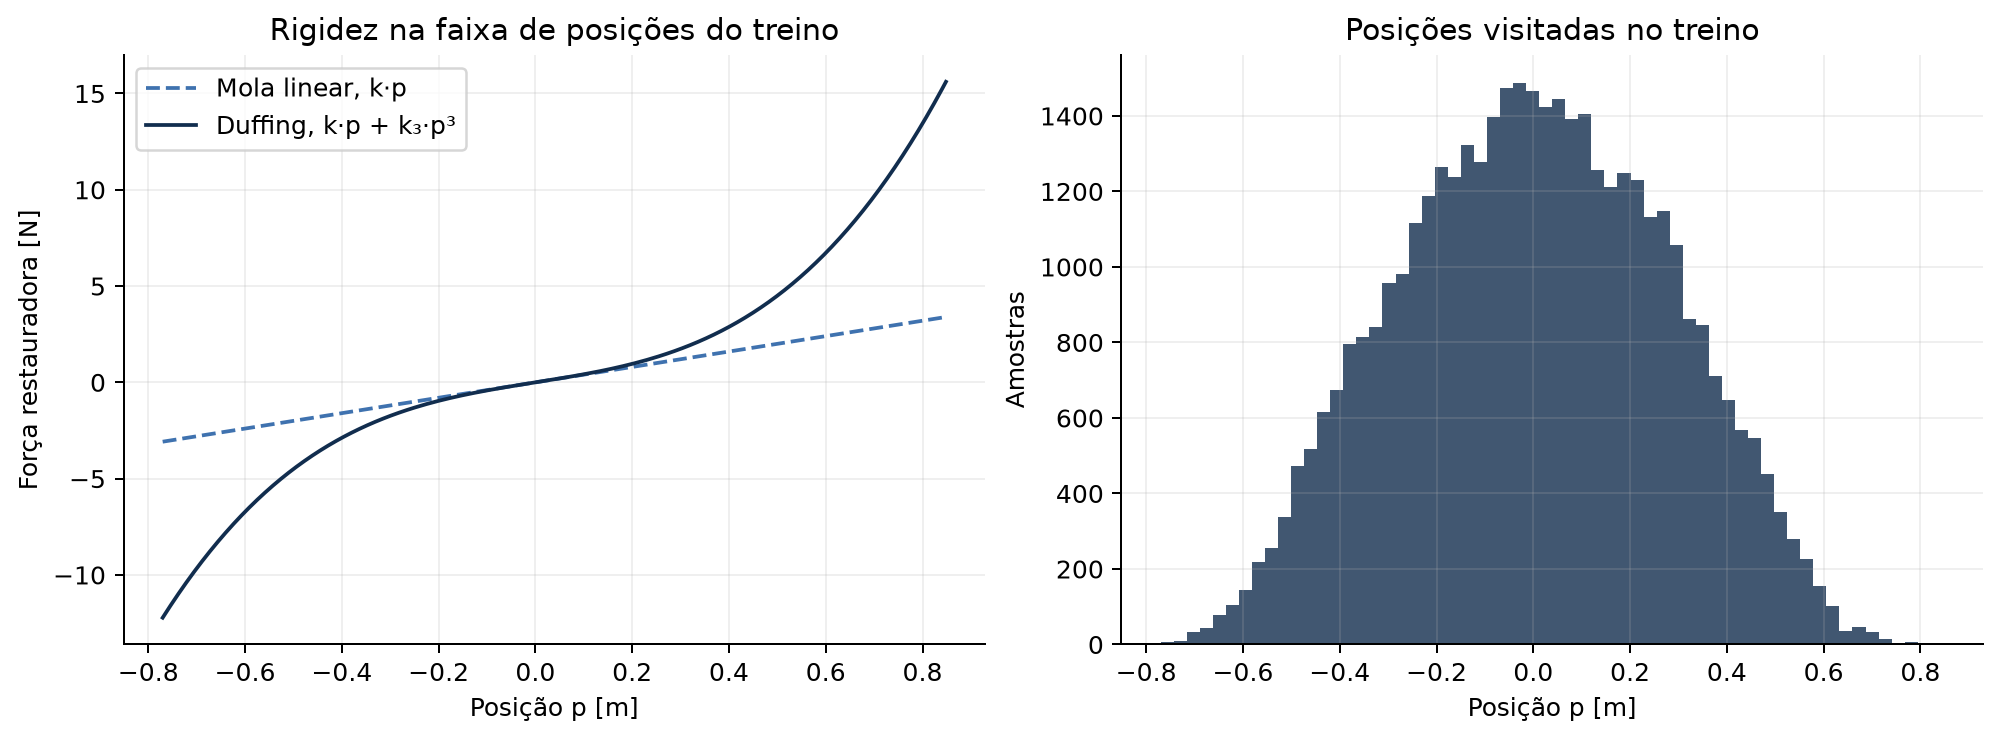
\includegraphics[width=\linewidth]{figuras/duffing-nao-linearidade.png}
\caption{E003. Esquerda: força restauradora da mola de Duffing comparada à parte linear, na faixa
de posições do treino. Direita: distribuição das posições visitadas no treino.}\label{fig:duffing}
\end{figure}

Dados, divisão, origens, critérios e rede são os mesmos do E002, a menos da planta e da excitação.
A Tabela~\ref{tab:duffing} resume o teste.

\begin{table}[ht]
\centering
\caption{E003, Duffing sem ruído: RMSE da trajetória simulada no teste [m]. Rede: média $\pm$
desvio-padrão de três sementes.}\label{tab:duffing}
\small\setlength{\tabcolsep}{4pt}
\begin{tabular}{lrrrr}
\toprule
Modelo & Parâmetros & 1 passo & 10 passos & 50 passos \\
\midrule
Persistência & 0 & \num{3.47e-2} & \num{2.04e-1} & \num{3.80e-1} \\
ARX(8,8) & 17 & \num{1.11e-5} & \num{8.37e-3} & \num{8.92e-2} \\
NARX(4,4), grau 3 & 165 & \num{4.3e-10} & \num{2.0e-9} & \num{5.5e-9} \\
Mamba-3 & \num{34949} & $(\num{0.89}\pm\num{0.25})\times10^{-3}$ & $(\num{6.07}\pm\num{1.88})\times10^{-3}$ & $(\num{1.53}\pm\num{0.61})\times10^{-2}$ \\
\bottomrule
\end{tabular}
\end{table}

Três observações:
\begin{itemize}\itemsep0pt
  \item \textbf{O ARX deixa de servir.} A validação escolheu a maior ordem da grade, ARX(8,8), e o erro
  em 50 passos chega a \SI{8,9}{cm}. Num diagnóstico posterior, ordens até 64 mantiveram o erro em
  cerca de \SI{8,8}{cm}: a limitação é de estrutura, não de ordem.
  \item \textbf{O NARX polinomial aproxima o sistema quase até a precisão numérica, sem conter o
  sistema.} O mapa amostrado de uma equação diferencial com mola cúbica não é um polinômio finito das
  entradas e saídas passadas; o NARX de grau 3 com dois atrasos, que corresponderia à ``estrutura
  física'', erra \SI{1,4e-4}{m} na validação. O erro de $\num{5.5e-9}$\,m aparece com quatro
  atrasos, numa regressão mal condicionada (posto 137 de 165), e dois dos seis candidatos divergiram
  na simulação da validação. O grau máximo da grade (3) também foi escolhido sabendo que a mola é
  cúbica, o que favorece o NARX.
  \item \textbf{A rede fica entre os dois}: $(\num{1.53}\pm\num{0.61})$\,cm em 50 passos, de 4 a 8
  vezes menos que o ARX conforme a semente, sem nenhuma informação sobre a forma da não linearidade.
  Em termos relativos, o NRMSE passa de 2,4\,\% na planta linear para 5,4\,\% no Duffing.
\end{itemize}
O posto incompleto do NARX vem em boa parte da excitação: com patamares de pelo menos cinco amostras,
vários produtos de entradas atrasadas são sempre nulos (só os monômios da entrada têm posto 22 de
35). O sinal não excita persistentemente todos os regressores, e nenhum modelo foi avaliado com
entradas que mudam a cada amostra, como as que um MPC produziria.
O ensaio também mostra por que a simulação é o critério relevante para o uso pretendido: em um passo, o ARX(8,8) erra
\emph{menos} que a rede ($\num{1.1e-5}$ contra $\num{8.9e-4}$\,m), porque oito atrasos de um sinal
suave permitem extrapolar bem uma amostra adiante. O erro do modelo errado só aparece quando ele
realimenta as próprias previsões.

\subsection{E004: Duffing com ruído de medição}

O E004 repete o E003 com uma única mudança: ruído gaussiano branco de desvio-padrão \SI{2}{cm} somado
à posição medida, em todos os conjuntos. As trajetórias de força e de posição verdadeira são as
mesmas do E003. O desvio-padrão da posição é de cerca de \SI{28}{cm}, uma relação sinal-ruído de
aproximadamente 14 em amplitude. Os modelos só veem a medição ruidosa: ajuste, normalização, escolha
na validação e condições iniciais de cada simulação usam a posição com ruído. No teste, as mesmas
previsões são comparadas também com a posição sem ruído, guardada à parte, que mede quão bem cada
modelo reproduz a planta (Tabela~\ref{tab:ruido}).

\begin{table}[ht]
\centering
\caption{E004, Duffing com ruído de medição (desvio de \SI{2}{cm}): RMSE da trajetória simulada no
teste [m], medido contra a posição \emph{sem ruído}. Entre parênteses, o RMSE de 50 passos contra a
medição ruidosa, que tem piso de cerca de \SI{0,02}{m}.}\label{tab:ruido}
\small\setlength{\tabcolsep}{4pt}
\begin{tabular}{lrrrr}
\toprule
Modelo & 1 passo & 10 passos & 50 passos & (medição) \\
\midrule
Persistência & \num{4.06e-2} & \num{2.04e-1} & \num{3.80e-1} & (\num{3.81e-1}) \\
ARX(8,8) & \num{1.84e-2} & \num{5.14e-2} & \num{1.02e-1} & (\num{1.04e-1}) \\
NARX(4,4), grau 3 & \num{2.46e-2} & \num{6.72e-2} & \num{1.45e-1} & (\num{1.46e-1}) \\
Mamba-3 & $(\num{9.1}\pm\num{0.3})\times10^{-3}$ & $(\num{1.13}\pm\num{0.12})\times10^{-2}$ & $(\num{1.54}\pm\num{0.28})\times10^{-2}$ & (\num{2.53e-2}) \\
\bottomrule
\end{tabular}
\end{table}

\begin{figure}[ht]
\centering
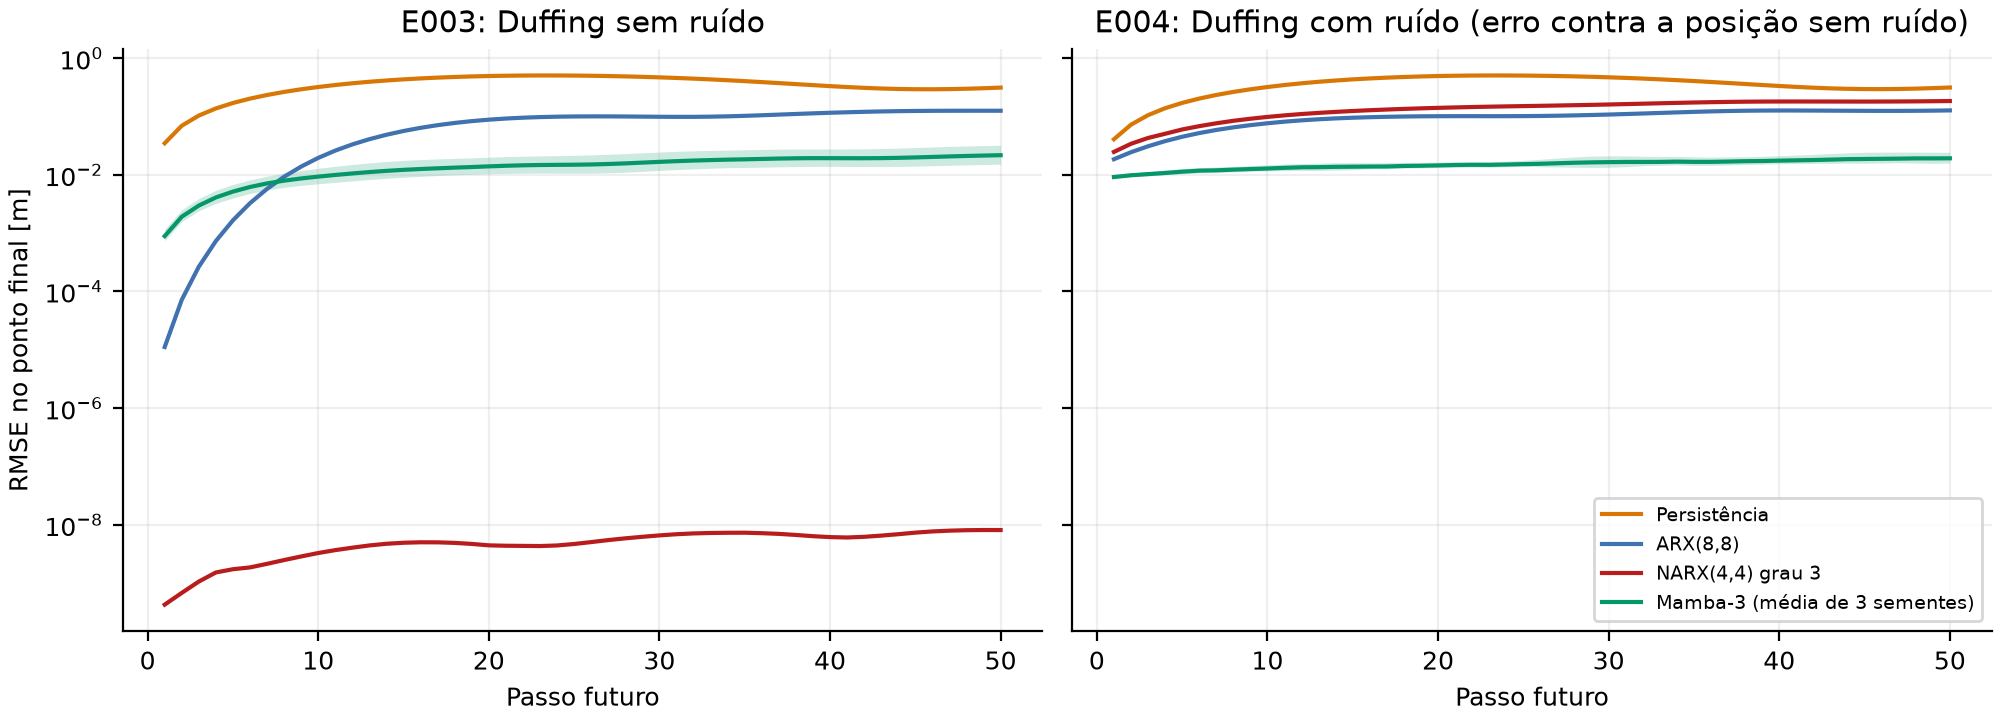
\includegraphics[width=\linewidth]{figuras/erro-horizonte-duffing.png}
\caption{Erro no passo futuro $h$ (RMSE sobre as 545 origens de teste), em escala logarítmica, para os
modelos escolhidos nas execuções registradas. No E004, o erro é medido contra a posição sem ruído.
Faixa verde: menor e maior valor entre as três sementes da rede. O NARX do E004 é o de quatro atrasos;
com mais atrasos ele se aproxima da rede (Tabela~\ref{tab:sensibilidade}).}\label{fig:horizonte}
\end{figure}

Na execução registrada, o quadro se inverte em relação ao E003: o NARX, que era quase exato, passa a
errar \SI{14,5}{cm} em 50 passos, mais que o ARX (\SI{10,2}{cm}), enquanto a rede mantém
praticamente o mesmo erro que tinha sem ruído (a diferença é menor que a dispersão entre sementes).
A rede erra 6,6 vezes menos que o ARX e 9,4 vezes menos que o NARX (de 5,5 a 10,6 vezes, conforme a
semente; Figura~\ref{fig:horizonte}). A Figura~\ref{fig:simulacao} mostra uma das 545 simulações.

\begin{figure}[ht]
\centering
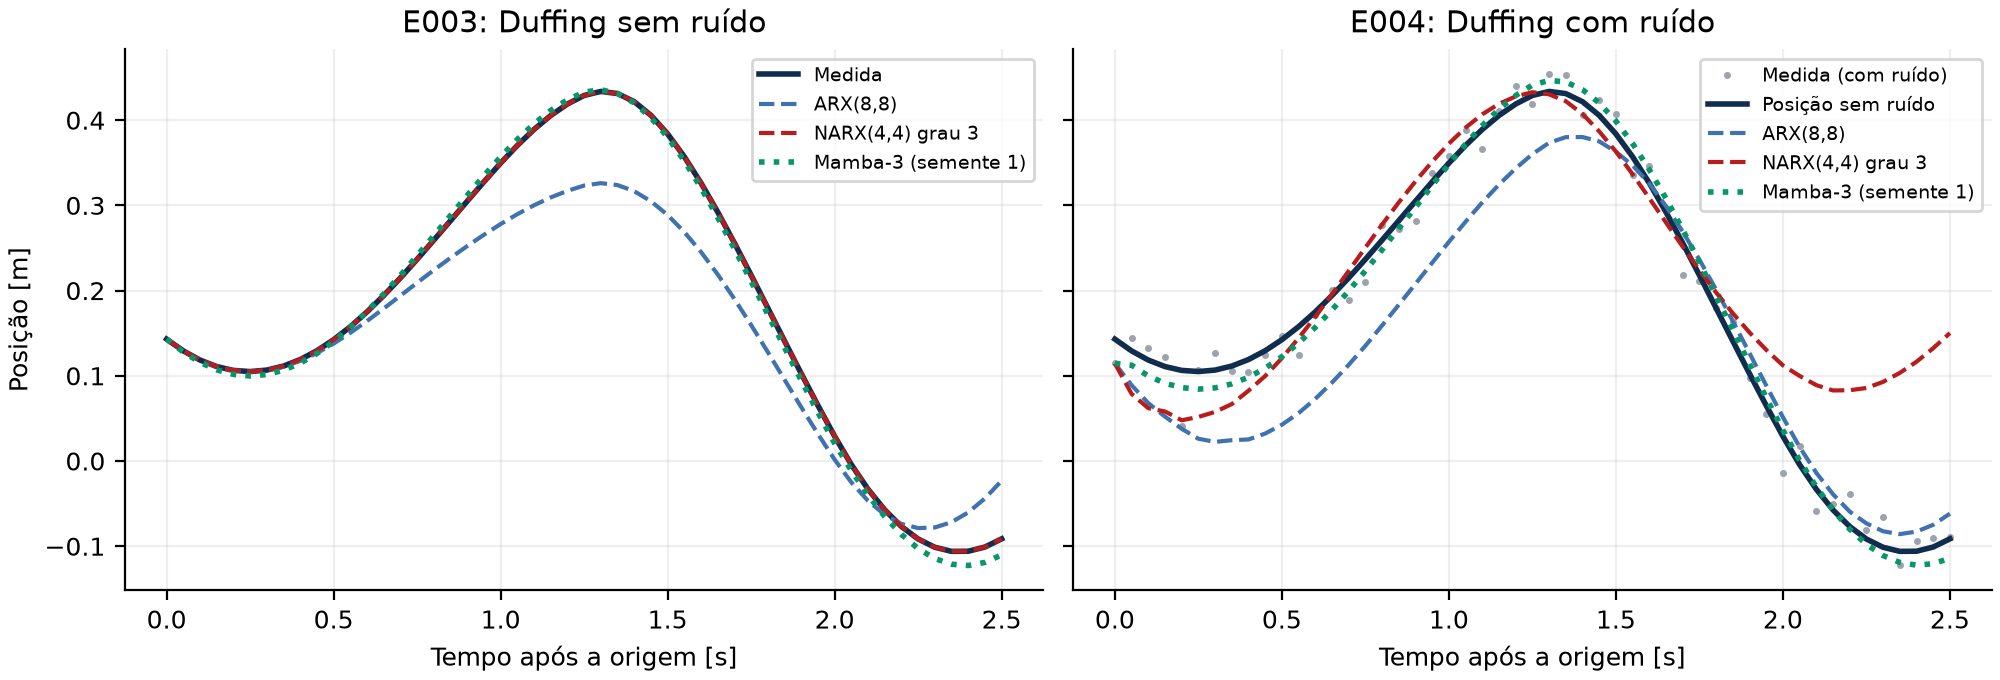
\includegraphics[width=\linewidth]{figuras/simulacao-duffing.png}
\caption{Simulação de 50 passos a partir da primeira origem da primeira trajetória de teste. Até a
origem, os modelos recebem medições; depois, só a força futura e as próprias previsões. Mesmo trecho
nos dois ensaios; à direita, as medições têm ruído.}\label{fig:simulacao}
\end{figure}

\paragraph{Essa vantagem não se sustenta.} Como o NARX escolhido estava na borda da grade
($n\le4$), fizemos um diagnóstico posterior ampliando apenas o número de atrasos, com o mesmo ajuste
e o mesmo critério de validação (Tabela~\ref{tab:sensibilidade}). Esse diagnóstico foi feito
\emph{depois} de conhecer o teste do E004; os valores de teste servem para entender o resultado, não
para escolher modelos.

\begin{table}[ht]
\centering
\caption{Diagnóstico posterior (E004): NARX de grau 3 com mais atrasos. RMSE da trajetória de 50
passos [m]; validação contra a medição ruidosa (critério do protocolo), teste contra a posição sem
ruído. ``Diverge'': valores não finitos na simulação.}\label{tab:sensibilidade}
\small\setlength{\tabcolsep}{5pt}
\begin{tabular}{lrrrrrrr}
\toprule
 & $n=4$ & $n=5$ & $n=6$ & $n=8$ & $n=10$ & $n=12$ & Mamba-3 \\
\midrule
Parâmetros & 165 & 286 & 455 & 969 & \num{1771} & \num{2925} & \num{34949} \\
Validação & \num{0.149} & \num{0.097} & \num{0.062} & \num{0.034} & \num{0.027} & \num{0.025} & \num{0.025} \\
Teste & \num{0.145} & \num{0.094} & \num{0.059} & \num{0.029} & \num{0.019} & diverge & \num{0.015} \\
\bottomrule
\end{tabular}
\end{table}

Com mais atrasos, o erro do NARX cai rapidamente: com $n=10$, chega a \SI{1,9}{cm} no teste,
dentro da faixa das sementes da rede (1,4 a \SI{1,9}{cm}). Com $n=12$, o modelo empata com a rede
na validação e seria o escolhido pelo protocolo, mas diverge no teste; com $n=14$, diverge já na
validação. A vantagem da execução registrada é, portanto, um artefato do limite da
grade. O que o E004 mostra é outra coisa:
\begin{itemize}\itemsep0pt
  \item O erro do NARX pequeno vem sobretudo de \textbf{coeficientes enviesados}: o ajuste por mínimos
  quadrados de um passo usa saídas passadas ruidosas como se fossem exatas~\cite{ljung1999,
  billings2013}. O mesmo NARX(4,4), simulado a partir de condições iniciais sem ruído, ainda erra
  \SI{14,3}{cm}.
  \item A \textbf{condição inicial} também pesa: o NARX(4,4) ajustado aos dados \emph{sem} ruído,
  quase exato no E003, erra \SI{5,1}{cm} quando parte de quatro medições ruidosas. A rede, que é
  aquecida com 256 medições, estima melhor o estado inicial. Parte da sua vantagem vem dessa
  filtragem, que os métodos tradicionais também podem ter, com estimação do estado inicial ou um
  observador, mas que não demos a eles.
  \item O NARX de ordem alta compensa o ruído com milhares de termos, mas é \textbf{numericamente
  frágil}: a validação não protege contra divergência no teste.
\end{itemize}

\subsection{O que os ensaios mostram}

Lidos em conjunto, os quatro ensaios sustentam três afirmações e deixam uma em aberto:
\begin{enumerate}\itemsep0pt
  \item Com o mesmo tamanho, o mesmo treino e nenhuma informação sobre a planta, a rede Mamba-3
  identificou os três cenários sem divergir, com NRMSE de simulação de 50 passos de 2,4\,\% (linear)
  e 5,4 a 5,5\,\% (Duffing, com e sem ruído).
  \item Quando a classe tradicional representa bem o sistema e os dados são limpos (ARX na planta
  linear, NARX cúbico no Duffing), o método tradicional é muito mais preciso e barato: ajuste em menos
  de \SI{0,2}{s}, contra cerca de \SI{4}{min} por treino da rede e 33 a \SI{38}{min} pela busca
  completa (três taxas de aprendizado e três sementes).
  \item Quando a classe tradicional não representa o sistema (ARX no Duffing), a rede é bem melhor.
  \item Com ruído, a comparação com o NARX depende da amplitude da grade e do tratamento da condição
  inicial. Os dados atuais \textbf{não} mostram vantagem da rede sobre um NARX de ordem suficiente,
  mas mostram que esse NARX fica frágil.
\end{enumerate}

\paragraph{Limitações.}
\begin{itemize}\itemsep0pt
  \item \textbf{Escopo dos dados:} plantas simuladas de baixa ordem, um único nível de ruído e
  excitação por patamares, que não excita persistentemente todos os regressores polinomiais.
  \item \textbf{Grades das referências clássicas:} ficaram na borda nos dois casos, e o grau máximo do
  NARX foi escolhido sabendo que a planta é cúbica. Os modelos tradicionais não tiveram estimação do
  estado inicial, ajuste pelo erro de simulação nem modelo de ruído.
  \item \textbf{Rede:} uma só configuração de tamanho, treinada apenas com erro de um passo e,
  provavelmente, por pouco tempo (os melhores \emph{checkpoints} ficaram entre as épocas 240 e 300,
  de 300).
  \item \textbf{Estatística e uso do teste:} três sementes e cinco trajetórias de teste, com origens
  sobrepostas, e sem intervalos de confiança. O E004 foi planejado depois de ver o teste do E003, sobre
  as mesmas trajetórias, e o diagnóstico da Tabela~\ref{tab:sensibilidade} usou o teste do E004.
  \item \textbf{Implementação e referências:} o Mamba-3 não foi comparado com os \emph{kernels}
  oficiais, e não há comparação com outras redes recorrentes (LSTM, GRU). Por isso o resultado ainda
  não pode ser atribuído às SSMs em particular.
\end{itemize}

% ---------------------------------------------------------------------------
\section{Tese do trabalho}\label{sec:tese}

Até o relatório 1, o trabalho tinha um tema, mas não uma tese: ``usar SSMs para identificar e
controlar sistemas'' não diz o que se espera mostrar nem o que contaria como resultado negativo.
Com o redirecionamento combinado com o orientador e a evidência dos ensaios, propomos a seguinte
formulação, a ser confirmada na apresentação:

\begin{quote}
\textbf{Tese.} Um modelo de espaço de estados estruturado e seletivo (Mamba-3), treinado apenas com
dados de entrada e saída, é uma estratégia \emph{viável} de identificação caixa-preta de sistemas
dinâmicos para previsão de vários passos. Ele não supera os métodos tradicionais quando a classe de
modelos destes representa bem o sistema e os dados são limpos. Ele é \emph{interessante} se, nos
cenários em que os métodos tradicionais exigem escolhas cuidadosas (ordem, termos, tratamento do
ruído e do estado inicial), alcançar erro igual ou menor com um procedimento de ajuste padronizado e
a um custo aceitável, e se essa vantagem for própria das SSMs, e não de qualquer rede recorrente.
\end{quote}

A tese se desdobra em três hipóteses, avaliadas sempre com os mesmos dados, a mesma divisão, o mesmo
critério de escolha na validação e a mesma simulação de 50 passos no teste. Os limiares abaixo foram
fixados depois dos ensaios deste relatório; valem como critério, sem alterações, para os ensaios
seguintes:
\begin{description}\itemsep0pt
  \item[H1 -- viabilidade.] Em todos os sistemas avaliados, a rede atinge NRMSE de simulação de 50
  passos de no máximo 10\,\% no teste, sem valores não finitos em nenhuma semente.
  \item[H2 -- limite.] Quando a classe tradicional representa bem o sistema e não há ruído, o método
  tradicional tem erro menor que a rede e custo de ajuste ao menos cem vezes menor.
  \item[H3 -- interesse.] Em pelo menos um cenário com ruído, não linearidade não polinomial ou dados
  reais, o erro médio da rede é menor que o do melhor método tradicional e o da melhor rede recorrente
  de referência (GRU). Os competidores são escolhidos na validação, a partir de grades definidas antes
  de ver os dados e sem usar conhecimento da planta. A diferença precisa superar a incerteza, estimada
  por \emph{bootstrap} sobre as trajetórias de teste e pela dispersão entre sementes; dentro dessa
  margem, os resultados são considerados equivalentes.
\end{description}

\noindent\textbf{O que a evidência atual diz.}
\begin{itemize}\itemsep0pt
  \item \textbf{H1} é sustentada: NRMSE entre 2,4 e 5,5\,\% nos três cenários, sem divergência.
  \item \textbf{H2} também: ARX na planta linear e NARX no Duffing sem ruído foram muito mais precisos,
  e seu ajuste levou menos de \SI{0,2}{s}, contra minutos de treino da rede.
  \item \textbf{H3 está em aberto.} Contra o ARX no Duffing, a rede é bem melhor, mas o ARX é uma
  referência fraca para uma planta não linear. Contra o NARX com ruído, a vantagem inicial desapareceu
  quando a grade foi ampliada (seção~\ref{sec:ensaios}). Ainda não há referência recorrente, grade
  definida antes de ver os dados nem estimativa de incerteza.
\end{itemize}

A tese pode ser refutada, e isso também seria um resultado do TCC. Se referências tradicionais bem
ajustadas, ou uma GRU, igualarem ou superarem a rede de forma consistente nos cenários de H3, a
conclusão será que, para sistemas pequenos com uma entrada e uma saída, as SSMs não trazem vantagem
que justifique seu custo. Por isso o cronograma (seção~\ref{sec:cronograma}) prioriza fortalecer as
referências antes de ampliar a rede.

% ---------------------------------------------------------------------------
\section{Cronograma até a entrega final}\label{sec:cronograma}

O cronograma do relatório 1 previa escolher o sistema e o método de comparação até 18/10 e obter
as primeiras previsões até 01/11; as duas etapas foram concluídas, e a comparação com referências
não lineares, prevista para novembro, foi antecipada (E003 e E004). Com o novo recorte, as etapas de
controle saem do cronograma e dão lugar a ensaios que testem a tese.

\begin{table}[ht]
\centering\small
\begin{tabularx}{\linewidth}{@{}p{2.6cm}Y@{}}
\toprule
Período & Atividades e resultados esperados \\
\midrule
27/10 & Apresentação; registrar o retorno do orientador e da banca sobre a tese e o recorte. \\
28/10 a 08/11 & \textbf{Protocolo e referências mais justos.} Fixar, antes de rodar, as grades de
todas as famílias, sem usar conhecimento da planta (atrasos até 16, grau até 4). Estimar o estado
inicial dos modelos tradicionais com a mesma janela de 256 medições usada pela rede. Ajustar o NARX
também pelo erro de simulação e com seleção de termos (mínimos quadrados ortogonais) e incluir uma
GRU com o mesmo protocolo. Treinar a rede por mais tempo e também com perda de vários passos.
Reservar um conjunto de teste novo, usado uma única vez no fim, e calcular intervalos por
\emph{bootstrap}. Repetir E003 e E004 nessas condições. \\
09 a 15/11 & \textbf{Onde a estrutura não ajuda.} Não linearidade que não é polinomial (por exemplo,
saturação ou atrito), excitação que muda a cada amostra (multisseno) e varredura do nível de ruído e
da quantidade de dados de treino. Resultado: curvas de erro em função do ruído e dos dados para cada
família. \\
16 a 22/11 & \textbf{Dados reais.} \emph{Benchmark} Silverbox~\cite{wigren2013}, circuito eletrônico que
implementa um oscilador do tipo Duffing, comparando com os resultados publicados de métodos
tradicionais. Resultado: primeira evidência fora de simulação. \\
23 a 29/11 & Custo computacional (treino e simulação de muitas trajetórias), consolidação das tabelas,
verificação da implementação do Mamba-3 contra os \emph{kernels} oficiais numa GPU NVIDIA, se houver
acesso. Encerrar novos experimentos. \\
30/11 a 06/12 & Redação do relatório final, revisão pelo grupo e pelo orientador, ensaio da
apresentação presencial. \\
07/12 e 08/12 & Entrega do relatório final e apresentação presencial (datas a confirmar no Moodle). \\
\bottomrule
\end{tabularx}
\end{table}

Se sobrar tempo, o uso do modelo identificado como preditor num MPC simples pode entrar como
demonstração, sem ser critério de sucesso do trabalho.

% ---------------------------------------------------------------------------
\begin{thebibliography}{99}\small\itemsep0pt

\bibitem{cevaal2026} CEVAAL, M.; DE JONG, T. O.; LAZAR, M. \emph{Mamba Sequence Modeling meets Model
Predictive Control}. arXiv:2604.13857, versão 2, 28 set. 2026. Disponível em:
\url{https://arxiv.org/abs/2604.13857}.

\bibitem{gu2022s4} GU, A.; GOEL, K.; RÉ, C. \emph{Efficiently Modeling Long Sequences with
Structured State Spaces}. ICLR, 2022. Disponível em: \url{https://arxiv.org/abs/2111.00396}.

\bibitem{gu2023mamba} GU, A.; DAO, T. \emph{Mamba: Linear-Time Sequence Modeling with Selective State
Spaces}. 2023; versão revisada em 2024. Disponível em: \url{https://arxiv.org/abs/2312.00752}.

\bibitem{gu2020hippo} GU, A.; DAO, T.; ERMON, S.; RUDRA, A.; RÉ, C. \emph{HiPPO: Recurrent Memory
with Optimal Polynomial Projections}. NeurIPS, 2020. Disponível em:
\url{https://arxiv.org/abs/2008.07669}.

\bibitem{lahoti2026mamba3} LAHOTI, A.; LI, K. Y.; CHEN, B.; WANG, C.; BICK, A.; KOLTER, J. Z.; DAO, T.;
GU, A. \emph{Mamba-3: Improved Sequence Modeling using State Space Principles}. arXiv:2603.15569, 2026. Disponível em: \url{https://arxiv.org/abs/2603.15569}.

\bibitem{mambarepo} STATE-SPACES. \emph{mamba} (repositório de código, licença Apache-2.0),
\emph{commit} \texttt{e9594ce1c732d97440f0332fdc43170a2294dbfa}, 22 jul. 2026. Disponível em:
\url{https://github.com/state-spaces/mamba}. Acesso em: 17 out. 2026.

\bibitem{ljung1999} LJUNG, L. \emph{System Identification: Theory for the User}. 2. ed. Upper Saddle
River: Prentice Hall, 1999.

\bibitem{wigren2013} WIGREN, T.; SCHOUKENS, J. Three free data sets for development and benchmarking in
nonlinear system identification. In: \emph{European Control Conference (ECC)}, 2013.

\bibitem{billings2013} BILLINGS, S. A. \emph{Nonlinear System Identification: NARMAX Methods in the
Time, Frequency, and Spatio-Temporal Domains}. Chichester: Wiley, 2013.

\end{thebibliography}

\end{document}
